% !TeX root = ../../main.tex
\section{Corporate overview}
\subsection{Plant location}
\label{sec:location}
AHP and TOPSIS methodologies were used to determine a suitable country for Nitroma’s chemical plant. The key factors taken into consideration are summarised in Appendix \ref{app:location}. China was identified as the optimal country for Nitroma's plant, owing to its strong local supply of toluene and low business operating costs. China is also the world’s fastest growing herbicides market and the second fastest growing dye and pharmaceutical market, resulting in a favourable demand of Nitroma’s products. To identify a suitable city within China, the spread of toluene suppliers, access to distribution channels, local market demand and business policies across the provinces of China were studied. The Nanjing Chemical Industry Park in Nanjing, Jiangsu was selected as the location of Nitroma’s plant. China’s largest toluene manufacturer, operated by Sinopec Yangzi Petrochemical, is situated within 10 km of Nitroma’s selected site in Jiangsu \cite{sinopec_group_sinopec_2014}. The site is also located 40 km away from the main Nanjing city, as per Lees' safety guidelines \cite{lees_lees_2012}. Moreover, the chosen location will allow Nitroma easy access to fresh water from the Jiajiang tributary of the Yangtze River less than 10 km away. Overall, the Jiangsu province hosts \SI{20}{\percent} of China’s inland waterways and 4710 km of highways, creating reliable access to buyers within the province and large markets in Zhejiang and Shanghai \cite{britannica_jiangsu_nodate}. Moreover, Jiangsu operates a favourable policy towards foreign-invested enterprises \cite{hktdc_sourcing_market_2008}.

\subsection{Mode of operation: Foreign-invested enterprise}
\label{sec:mode-of-operation}
Nitroma will establish itself as a foreign-invested enterprise (FIE) in China, in line with the Foreign Investment Law 2020 \cite{jones_day_china_2020}. As such, Nitroma will be incorporated under Chinese laws, with its equity investment coming from foreign investors and debt investment coming from Chinese commercial banks (\ref{sec:de-ratio}). As an FIE, Nitroma will have independent management of its processes, making it easier to negotiate contracts with buyers and suppliers. Being the innovator of a continuous liquid-phase nitration process, Nitroma will enjoy the benefit of owning intellectual property under its own name without sharing trade secrets with a local partner. Nitroma will not need to share profits either. 

In recent times, China has adopted an increasingly open stance towards foreign business as part of an effort to gain allies in its trade war against the US and to globalize its domestic industries \cite{cheng_chinas_2020}. The 2014 deal between INEOS and China’s state-run Sinopec to build a phenol plant in Nanjing, China is evidence of government interest in harnessing foreign capabilities for the enhancement of local industry \cite{pwc_new_2011}. Opportunities for favourable tax treatments also exist under new government policies in China, with the chemical raw material and products manufacturing industry being listed in the Ministry of Commerce’s Catalogue of Encouraged Foreign Investment Industries \cite{ministry_of_commerce_china_catalouge_2020}. 

The risks associated with the decision to operate as an FIE include cultural obstacles, buyer bias, language barriers, and lengthy wait times for governmental approvals. To tackle these risks, Nitroma will hire an entirely local labour force and implement a marketing strategy that will build consumer trust.

\subsection{Product line capacity}
\label{sec:product-capacity}
Nitroma’s plant capacity has been designed based on the local product demand and competitive landscape in China. In its first 5 years of operation, Nitroma aims to achieve the average industry market shares for PABA, PABH and OTOL respectively. Based on the estimated 2020 market, this is equivalent to 100, 539 and 652 tonnes yr\textsuperscript{-1} of PABA, PABH and OTOL respectively. In its first 5 years, the plant will operate for 275 days per year.

As an entrant into the Chinese chemicals industry where most buyers are locked into existing contracts with suppliers, Nitroma recognises the challenge of acquiring market share. Previous instances of failed market entries in China, like eBay’s expansion into the Chinese electronics market, have made Nitroma wary of a large-scale launch into a highly competitive industry \cite{obrien_4_2015}. However, Nitroma believes it can capture the average industry market share in its first 5 years of operation due to its unique competitive advantage and pricing strategy (discussed in Sections \ref{sec:pricing-strategy} and \ref{sec:USP}). Being an FIE, Nitroma also acknowledges the importance of utilising its first 5 years to develop rapport and build a local distribution network before expanding to a larger manufacturing scale. Details of plant expansion in line with the market growth of PABA, PABH and OTOL are discussed in \cref{sec:expansion}.

The initial operational capacity of 275 days per year has been carefully chosen to prevent overproduction based on market demand and Aspen modelling. Nitroma does not want to risk overproduction due to the consequent loss of profitability. In-built plant modularity will allow Nitroma to switch between the production of PABA (35 days/year) and PABH (240 days/year), whilst OTOL will always be produced (275 days/year). As suggested by Coulson \& Richardson, an additional 25 days per year are dedicated to planned shutdowns for maintenance, equipment cleaning and biannual renewals of catalyst \cite{sinnott_coulson_2005}. 

\subsection{Pricing strategy}
\label{sec:pricing-strategy}
Nitroma’s customer base is made up of price-sensitive dye, pharmaceutical, and agrochemical manufacturers who look for the cheapest supplier of raw material. Therefore, Nitroma will adopt a penetrative pricing strategy to enter the chemicals market in China. This strategy is designed to quickly attract customers to Nitroma and secure market share by offering lower prices \cite{corporate_finance_institute_penetrative_2021}. Being a capital-intensive business, a penetrative pricing strategy will also ensure that Nitroma is able to rapidly generate cash flow in order to meet its loan repayment targets and achieve a short payback period. Brand image or perceived brand quality are not important buying criteria for Nitroma’s customers, so a low price point will not damage Nitroma’s sales. Moreover, the strategy is expected to be effective because there is no differentiation in product features that may lure buyers to competitors.
%Furthermore, this strategy is expected to create goodwill between Nitroma and its buyers, who are likely to develop brand loyalty after discovering a high-value bargain (XX).

The average market prices of PABA, PABH, and OTOL were obtained from the quotes of various online Chinese suppliers (detailed in Section \ref{sec:price-agreement}).  Nitroma will price its three products \SI{12.5}{\percent} lower than the respective average market price, equivalent to \$25.80/kg for PABA, \$35.74/kg for PABH, and \$10.67/kg for OTOL. This price cut was chosen because it is the largest value that will not change Nitroma’s MCDM-based product selection (\cref{sec:product-selection}) and will still allow Nitroma to be priced above the cheapest supplier, reducing the likelihood of a price war. Moreover, a preliminary EP1 analysis showed that Nitroma is able to generate a healthy profit margin of \SI{64}{\percent} with this price cut – a positive indicator with reference to the industry average gross margins of \SI{21.20}{\percent}. 

It must be noted that Nitroma faces the risk of market backlash in the face of future price hikes as buyers may begin to expect permanently low prices. However, this is unlikely as Nitroma will only increase prices in-line with inflation and the Chinese Consumer Price Index (CPI). This move would not be profit-motivated. Further income escalation details are discussed in \cref{sec:cash-flows} - KEY ASSUMPTIONS.

\subsection{Unique selling points}
\label{sec:USP}
\paragraph{Cheap product}
Due to the continuous nature of Nitroma’s nitration process, the company will be able to utilise smaller equipment than traditional batch nitration operators that are prevalent in China \cite{lee_mordernizing_2015}. Nitroma will also require lesser utilities to support the nitration process as plant downtime and process inefficiencies will be reduced due to the continuous nature of the process. Therefore, Nitroma will have a lower CAPEX and OPEX than its competitors. Furthermore, Nitroma will enjoy the benefit of a reduced corporate tax rate of \SI{15}{\percent} because of operating as a foreign-invested company in a government-encouraged industry \cite{ministry_of_commerce_china_catalouge_2020}. As a result, Nitroma will be able to undercut its competitors on product price as discussed in \cref{sec:pricing-strategy}.

\paragraph{Reliable supply}
Following disasters like the deadly explosion in Chenjiagang Industrial Park in 2019, growing concerns around plant safety have led Chinese authorities to introduce upgraded safety laws \cite{naidu_china_2019}. Incumbents and newcomers in the Chinese chemicals market must adapt fast to survive the challenging phase of increased regulatory control. In 2019, Jiangsu shut down 9 chemical parks (equivalent to 1244 factories) due to safety risks \cite{kielburger_chinese_2019}. Nitroma seeks the reward of fulfilling unmet demand as many of its competitors are removed from the market. Nitroma’s inherently safe design means it is not threatened by closures, making it a more reliable supplier for buyers to enter long-term purchasing contracts with.
%For example, one policy has updated a 19-year-old manufacturing standard with new requirements for operating conditions on chemical sites (XX).

\subsection{Capacity expansion}
\label{sec:expansion}
As discussed in \cref{sec:product-capacity}, Nitroma will commence operations at 275 days per year in 2023. Given the maximum number of operating days available in a year are 340, this reflects an \SI{81}{\percent} initiating capacity. Every 5 years up to 2043, Nitroma will increase its capacity by an additional 10 days per year in line with the CAGRs of the P-ABA, P-ABH and O-TOL markets that are detailed in \cref{sec:market-analysis}.  This decision is motivated by Nitroma’s desire to retain a stable market share during its 20-year lifetime. Table \ref{tab:Expansion} summarises the projected results from Nitroma’s plant expansion.

\begin{table}[H]
\centering
\caption{Projected results of expansion}
\label{tab:Expansion}
\begin{tabular}{lr|cccc}
\toprule
\multicolumn{2}{l|}{\textbf{Year}}                & \textbf{2023} & \textbf{2028} & \textbf{2033} & \textbf{2038} \\\midrule
\textbf{Operating days} & \textit{BH production}  & 240           & 249           & 257.5         & 266           \\
\textbf{}               & \textit{BA production}  & 35            & 36            & 37.5          & 39            \\
\textbf{}               & \textit{\textbf{Total}} & \textbf{275}  & \textbf{285}  & \textbf{295}  & \textbf{305}  \\
\multicolumn{2}{r|}{\textbf{Capacity}}            & 81\%          & 84\%          & 87\%          & 90\%          \\\midrule
\textbf{Total output}   & \textit{P-ABA}          & 100           & 104           & 107           & 111           \\
\textbf{(tonnes/year)}  & \textit{P-ABH} & 539  & 557  & 577           & 596           \\
\textbf{}               & \textit{O-TOL}          & 652           & 676           & 699           & 723           \\
\textbf{}               & \textit{\textbf{Total}} & \textbf{1291} & \textbf{1337} & \textbf{1384} & \textbf{1431} \\
\multicolumn{2}{r|}{\textbf{Production increase}} & -             & 3.54\%        & 7.18\%        & 10.81\%       \\\midrule
\textbf{Nitroma}        & \textit{P-ABA}          & 1.4\%         & 1.4\%         & 1.4\%         & 1.4\%         \\
\textbf{market}         & \textit{P-ABH}          & 1.9\%         & 1.9\%         & 1.8\%         & 1.8\%         \\
\textbf{share (\%)}     & \textit{O-TOL}          & 0.2\%         & 0.2\%         & 0.2\%         & 0.2\%        \\\bottomrule
\end{tabular}
\end{table}


A very important assumption made in the calculation of these results is that the markets for Nitroma’s products will continue growing at the same rate as forecasted by analysts today. This is uncertain, and so, Nitroma has incorporated checkpoints on its business timeline to review market demand every 5 years (see \cref{sec:business-timeline}). If a further scale up is needed to meet market demand, Nitroma has the flexibility to increase capacity up to 340 operating days per year. Moreover, the ratio of operating days under BH production mode and BA production mode has been maintained at 240:35 (initiating level) over the lifetime of the plant. This is also subject to change based on market review checkpoints.
%A sensitivity analysis has been conducted on this critical ratio in Section XX.

To facilitate the expansion, Nitroma will not need to purchase new equipment or expand its plant area. However, raw material and utility costs will increase linearly with the number of operational days. The revenue from product sales will also grow proportionately. Therefore, Nitroma will not see any improvement in its profit margin although its profit will increase. The plant expansion has been represented in the company’s financial sheets found in Section XX.
%It should be noted that Nitroma aims to improve its profit margin by renegotiating contracts with suppliers to decrease the unit cost of raw material, but this is a point for future consideration by the company's procurement team. 

\subsection{Business timeline}
%\label{sec:business-timeline}
%\begin{figure}[h]
%\centering
 % 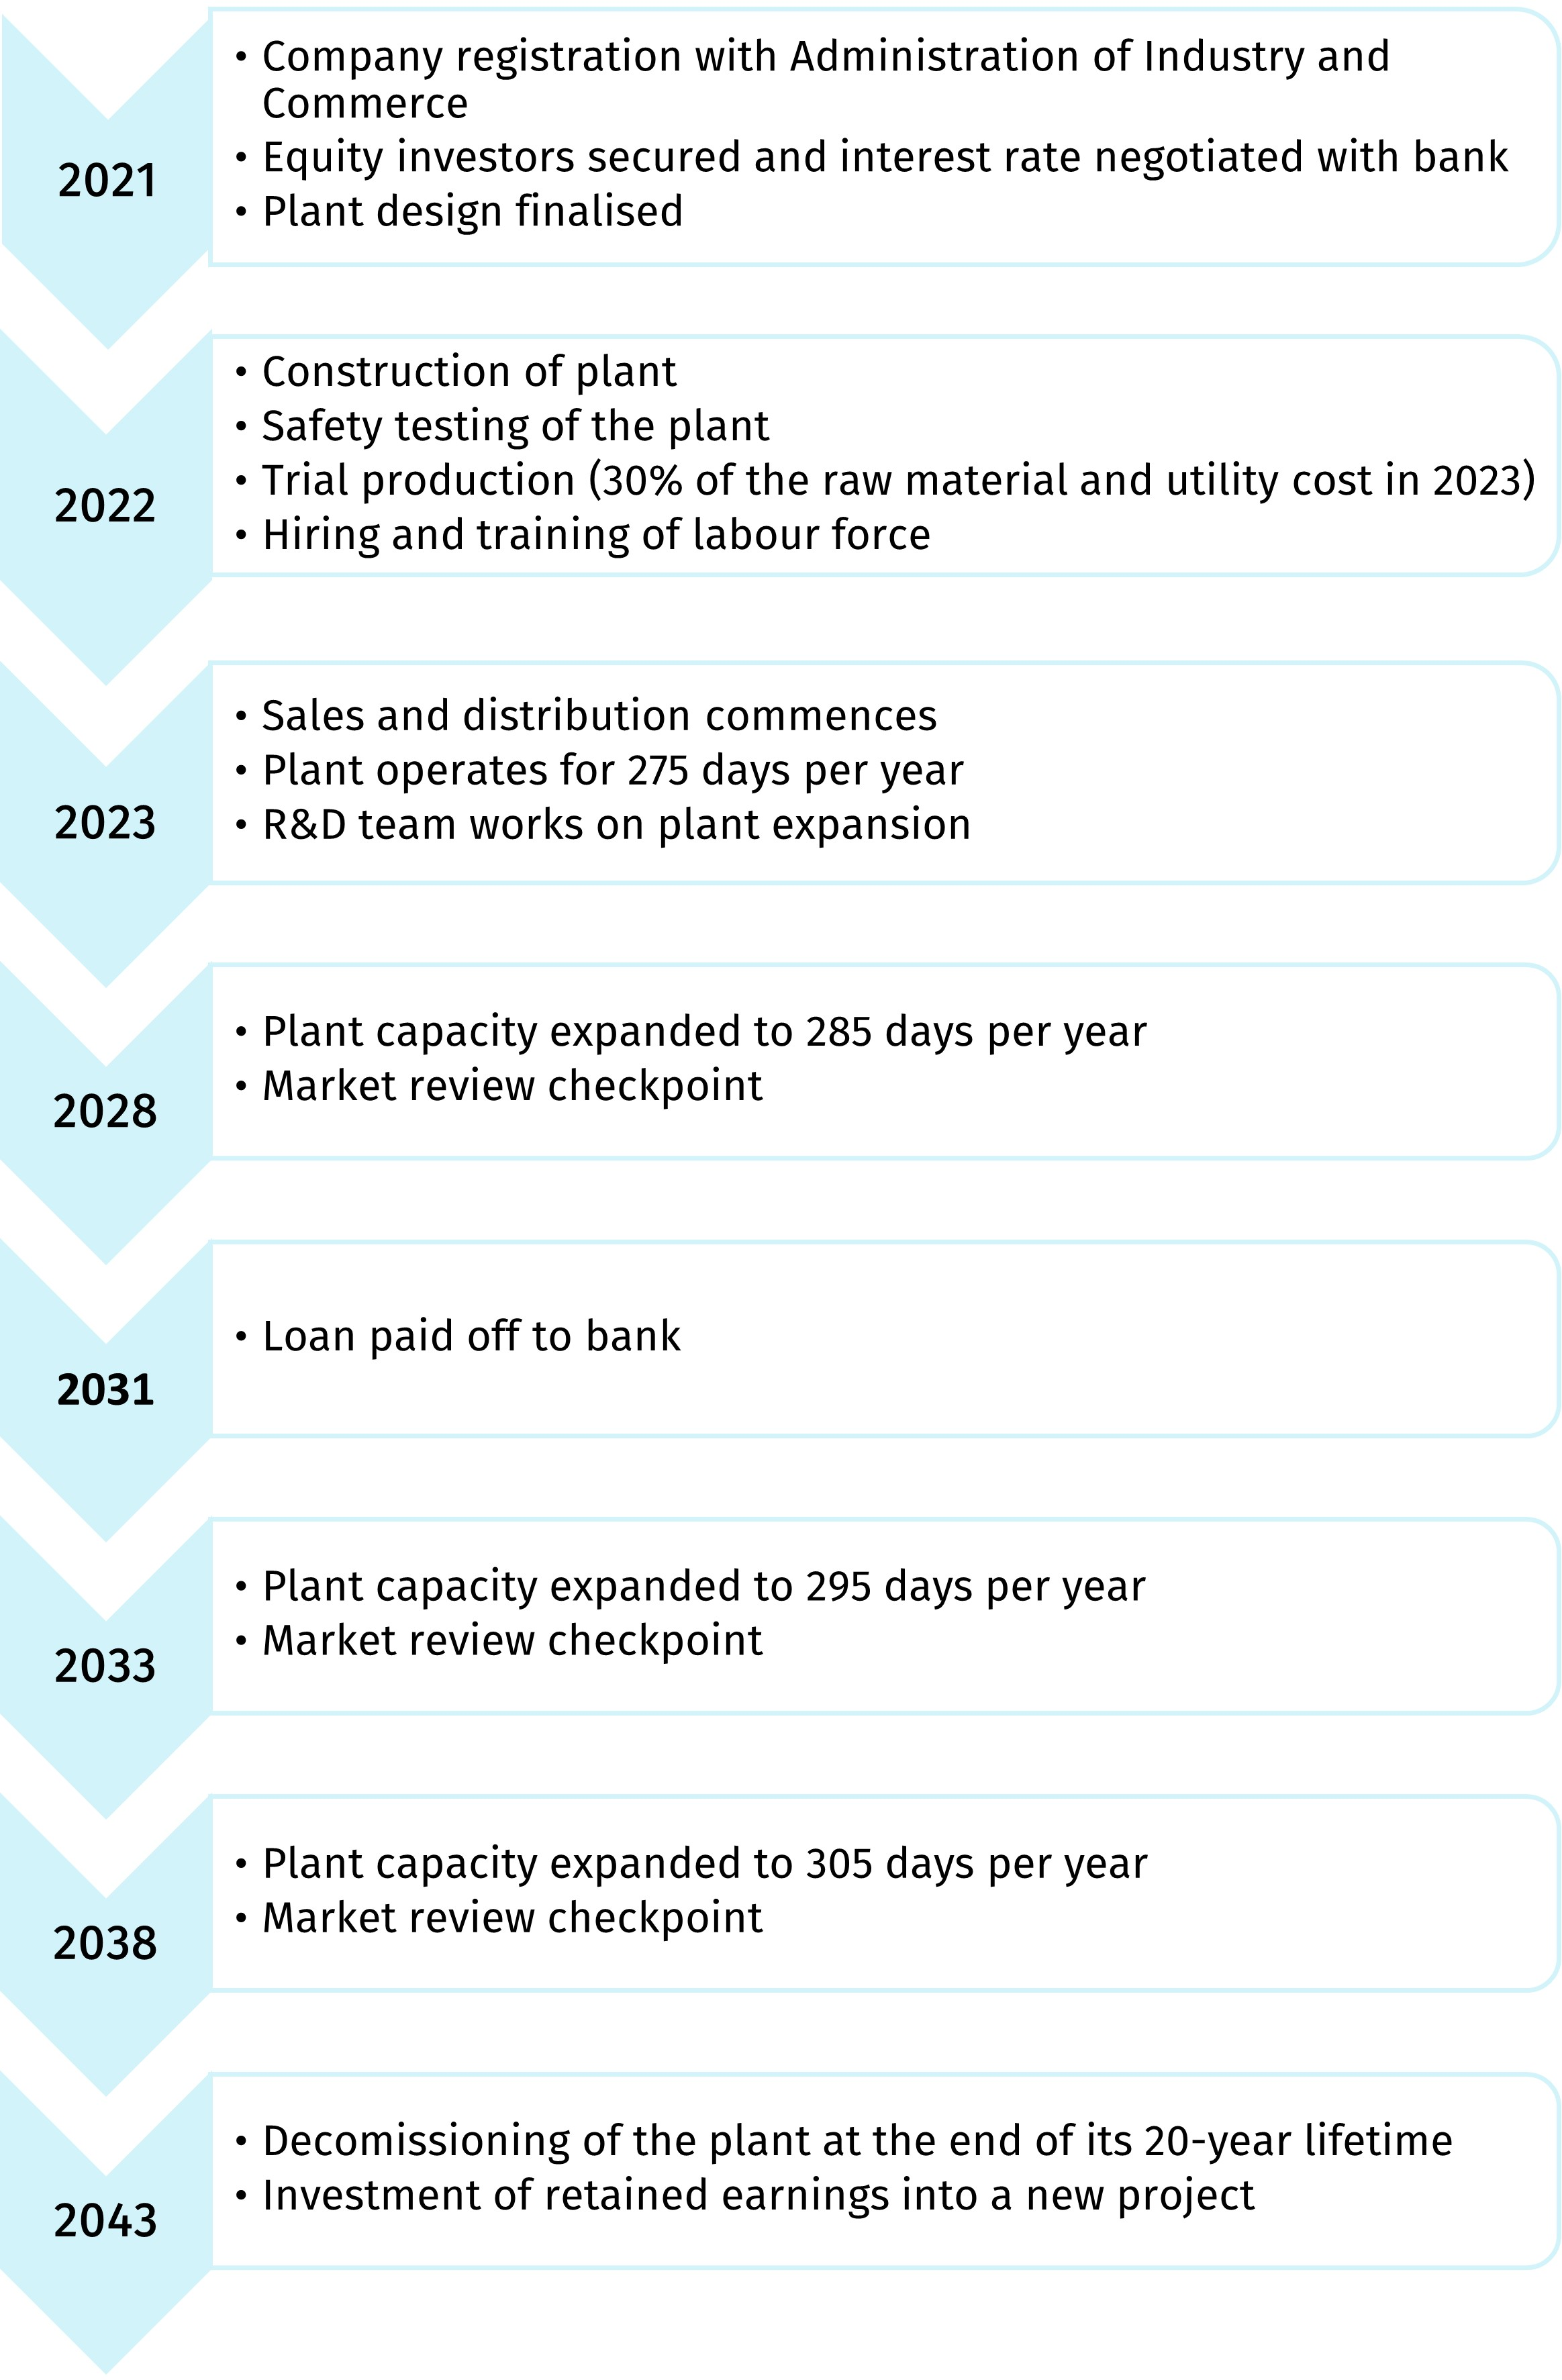
\includegraphics[width=12.5cm]{chapters/6-economics/figures/Business timeline.jpg}
 % \caption{Nitroma's business timeline}
 % \label{fig:business-timeline}
%\end{figure}

\subsection{External industry analysis: Porter's Five Forces}
\label{sec:five-forces}
Michael Porter’s Five Forces is a framework used to analyse a company’s external industry environment. The five forces represent threats to the company’s market position and profitability. The forces are scored 1 to 5, with 1 being Very Low Threat and 5 being Very High Threat. A major limitation of Porter’s Five Forces is that it is a static framework, meaning that it does not take any future changes into account. In reality, several forces, such as the bargaining power of suppliers, are likely to change over time. The combined results of all forces are summarised in Appendix \ref{app:five-forces} and discussed individually below.

\paragraph{Threat of substitute products}
Substitutes to Nitroma’s product line are limited because customers search for exact chemicals for their process designs. For example, OTOL is a specified essential raw material in the production of the herbicide metolachlor (). Changing raw material involves intensive R\&D along with a redesign of the process synthesis route, reactor units and downstream separation. This creates significant switching costs for the customer. The threat of substitute products would only become a strong force in the situation where customers switch their end product also. The average market price of product substitutes falls in the same range as the average market price of Nitroma’s product line, such as \meta-toluidine which costs \$8.90/kg (Zauba 2021). However, Nitroma will undercut the market with lower prices, mitigating the threat of cheaper substitutes.
%Alternate chemicals perform well in producing alternate dyes, agrochemicals, and pharmaceuticals, such as XX could be used to produce XX.

\begin{table}[H]
\centering
\caption{Thread of substitute products}
\label{tab:substitute-products}
\begin{tabular}{lccccc}
\toprule
\multirow{2}{*}{\textbf{Factor}} & Number of    & Performance of  & Price of         & Switching & Average \\
                                 & substitutes & substitutes  & substitutes & costs &         \\\midrule
\textbf{Score}                   & 1          & 2         & 2               & 1         & 1.5      \\\bottomrule
\end{tabular}%
\end{table}

\paragraph{Threat of new entrants}
The approximate capital cost of a chemical plant with a \SI{5000}{\tonne\per\year} capacity is \$5 million (based on data from Towler \& Sinnot), creating a steep barrier to entry \cite{sinnott_chemical_2020}. In order for chemical manufacturers to benefit from economies of scale, it is necessary for the process to be large scale. This makes it difficult for entrants to challenge an incumbent’s market position, who have already established large-scale operations. It is also difficult for entrants to make a differentiable chemical product. The nitration process itself, however, can be uniquely designed to enhance efficiency, safety, or cost savings. A high-level of technical expertise and industry know-how also prevents entrants from achieving an economical plant design. 
\begin{table}[H]
\centering
\caption{Threat of new entrants}
\label{tab:new-entrants}
\begin{tabular}{lccccc}
\toprule
\multirow{2}{*}{\textbf{Factor}} & Upfront    & Economies & Product         & Technical & Average \\
                                 & investment & of scale  & differentiation & knowledge &         \\\midrule
\textbf{Score}                   & 1          & 2         & 3               & 2         & 2      \\\bottomrule
\end{tabular}%
\end{table}

\paragraph{Bargaining power of buyers}
The customers of Nitroma’s product line consist of thousands of firms within the dye, pain relief drugs, and herbicides industries in China, representing a total annual market of \$24.5 billion (Mordor 2018, Vishal 20, Ken research 2020). Purchasing volume is spread evenly across firms within these industries, preventing one big buyer from dictating the terms of purchase. Therefore, customers carry little bargaining power. Nitroma’s three products are not differentiated from its competitors, meaning that customer loyalty is low beyond the scope of a contract and customers are sensitive to price. Moreover, customers are well-researched about the product because it serves as a raw material in their respective industries – this makes them better equipped to challenge unfair prices. Finally, buyers face low switching costs as there are numerous competitors producing the same products in China, as detailed in 
\cref{tab:market-summary}.

\begin{table}[H]
\centering
\caption{Bargaining power of buyers}
\label{tab:substitute-products}
\begin{tabular}{lcccccc}
\toprule
\multirow{2}{*}{\textbf{Factor}} & Number of    & Size of   & Buyer          & Price          & Switching & Average  \\
                                 & buyers       & order     & knowledge      & sensitivity    & costs     &          \\\midrule
\textbf{Score}                   & 1            & 1         & 3              & 4              & 4         & 2.6       \\\bottomrule
\end{tabular}%
\end{table}

\paragraph{Bargaining power of suppliers}
China is the largest supplier of toluene, methanol, formic acid, nitric acid, and hydrogen in Asia, with domestic production averaging 3.33m, 55m, 0.15m, 4.3m and 21m tonnes/year respectively (CCM 15, Yap 16, Guo 16, ICIS 2006, Jianjun 20). Whilst toluene is abundant and accessible in China, 5 key companies control over \SI{50}{\percent} of the supply (Yap 16). This grants them significant negotiating power. A similar situation exists for nitric acid (Guo 16). For the remaining raw materials, the number of suppliers is high and concentration of suppliers is low. For example, the largest methanol supplier in China, Shaanxi Yulin Energy Group Co., only produces \SI{8}{\percent} of the domestic supply (ICIS 2006). Moreover, there is little switching cost for Nitroma. However, Nitroma’s raw materials are common commodity feedstock for many industries, meaning suppliers have a large pool of clients to select from.

\begin{table}[H]
\centering
\caption{Bargaining power of suppliers}
\label{tab:supplier-power}
\begin{tabular}{lcccccc}
\toprule
\multirow{2}{*}{\textbf{Factor}} & Number of        & Concentration    & Quality of       & Competitive      & Switching     & Average   \\
                                 & suppliers        & of suppliers     & suppliers        & customers        & costs                     \\\midrule
\textbf{Score}                   & 1                & 3                & 1                & 3                & 1             & 1.8       \\\bottomrule
\end{tabular}%
\end{table}


\paragraph{Rivalry amongst exisiting competition}
The PABA, PABH and OTOL markets in China can be modelled most effectively by a perfect competition structure, where numerous small firms offer an undifferentiable product. The lack of a dominating company creates a low barrier for Nitroma to enter the industry. Existing competitors offer similar products, but without the promise of a consistent supply resulting from an inherently safe process design. The Chinese herbicide, dye and pain relief drug markets are also the fastest growing in Asia, with their CAGRs described in Section \ref{sec:market-analysis}. Therefore, Nitroma is advantageously positioned to capture a booming demand. Moreover, brand loyalty is low amongst consumers of Nitroma’s products who opt for the lowest prices. However, as a capital, research and asset intensive industry, there are fair barriers to exit. 
                                                        
\begin{table}[H]
\centering
\caption{Rivalry among existing competition}
\label{tab:rivalry}
\begin{tabular}{lcccccc}
\toprule
\multirow{2}{*}{\textbf{Factor}} & Number and size       & Industry   & Brand          & Barriers to    & Average   \\
                                 & of competitors        & growth     & loyalty        & exit           &           \\\midrule
\textbf{Score}                   & 2                     & 1          & 1              & 3              & 1.8       \\\bottomrule
\end{tabular}%
\end{table}

\subsection{Business risks: PESTEL}

% Please add the following required packages to your document preamble:
% \usepackage{multirow}
% \usepackage{graphicx}
% \usepackage[normalem]{ulem}
% \useunder{\uline}{\ul}{}
\begin{table}[H]
\centering
\caption{PESTEL analysis on Nitroma's business}
\label{tab:pestel}
\resizebox{\textwidth}{!}{%
\begin{tabular}{llll}
\toprule
\textbf{Factor}                & \textbf{Risk event}                                                                          & \textbf{Effect}                                                                                                                                                                                                                                                                                                                                                                                                                                                                                                                 & \textbf{Risk}                                       \\\midrule
\multirow{2}{*}{Political}     & \begin{tabular}[c]{@{}l@{}}Closure of  chemical \\ parks in China\end{tabular}               & \begin{tabular}[c]{@{}l@{}}In Jiangsu, increased safety legislation has led to the closure of 9 \\ chemical parks in 2019 (XX ). In Shandong, 25\% of chemical plants \\ have been shut (XX ). Some of these closed firms may be \\ customers or suppliers of   Nitroma, leading to a reduction in \\ Nitroma’s sales. Nitroma also faces the  threat of being shut if \\ unsafe practices are adopted by neighbouring factories within \\ Nanjing Chemical Industry Park.\end{tabular}                                         & \begin{tabular}[c]{@{}l@{}}S: H\\ L: M\end{tabular} \\ \cline{2-4} 
                               & US-China trade war                                                                           & \begin{tabular}[c]{@{}l@{}}Sanctions on US-China trade mean there is a smaller global \\ demand for the final products of Nitroma’s customers in the dye, \\ pharmaceutical and agrochemical sectors. This could \\ consequently affect Nitroma, which may experience reductions in \\ domestic sales volume.\end{tabular}                                                                                                                                                                                                      & \begin{tabular}[c]{@{}l@{}}S: M\\ L: L\end{tabular} \\ \hline
\multirow{2}{*}{Economic}      & \begin{tabular}[c]{@{}l@{}}Rise in interest\\ rates\end{tabular}                             & \begin{tabular}[c]{@{}l@{}}The People’s Bank of China is likely to toughen monetary policy in \\ order to prevent the unwanted effect of fuelling property price \\ gains and to deal with local shortage of pork (XX).   An increase in \\ interest rates would lead to higher IRR, cost of capital and\\ payback period for Nitroma.\end{tabular}                                                                                                                                                                             & \begin{tabular}[c]{@{}l@{}}S: M\\ L: M\end{tabular} \\ \cline{2-4} 
                               & \begin{tabular}[c]{@{}l@{}}Re-emergence of \\ coronavirus\end{tabular}                       & \begin{tabular}[c]{@{}l@{}}If the vaccine drive proves unsuccesful or new variants of \\ coronavirus emerge in China, another economic recession would \\ be inbound. Although this is not expected to affect the demand of \\ Nitroma's products, the plant would experience a loss of \\ productivty due to lockdown measures. A scenario analysis in \\ Section XX contains more details of this risk.\end{tabular}                                                                                                          & \begin{tabular}[c]{@{}l@{}}S: M\\ L: L\end{tabular} \\ \hline
\multirow{2}{*}{Social}        & \begin{tabular}[c]{@{}l@{}}Local attitude towards\\ foreign company\end{tabular}             & \begin{tabular}[c]{@{}l@{}}Because China has a long history of being exploited by foreign \\ countries, there is a local bias against dealing with foreign \\ businesses. As an FIE, Nitroma may have trouble in acquiring \\ a customer base.\end{tabular}                                                                                                                                                                                                                                                                     & \begin{tabular}[c]{@{}l@{}}S: H\\ L: M\end{tabular} \\ \cline{2-4} 
                               & Chinese “brain-drain”                                                                        & \begin{tabular}[c]{@{}l@{}}Brain drain is a term used for immigration of skilled labour away \\ from a country. China hosts the world’s highest ratio of students \\ who study abroad but never return home (XX). This loss of skilled \\ labour could result in a weak labour supply for Nitroma. As a \\ result, Nitroma may experience loss of productivity.\end{tabular}                                                                                                                                                    & \begin{tabular}[c]{@{}l@{}}S: M\\ L: M\end{tabular} \\ \hline
\multirow{2}{*}{Technological} & Weak IP laws                                                                                 & \begin{tabular}[c]{@{}l@{}}IP rights have been notoriously difficult to enforce in China. The \\ country is amongst 13 others on the US Trade Office’s Priority \\ Watch List 2015 (XX). Nitroma may suffer financial losses if its \\ novel liquid-phase continuous nitration process design is \\ counterfeited by local companies.\end{tabular}                                                                                                                                                                              & \begin{tabular}[c]{@{}l@{}}S: M\\ L: M\end{tabular} \\ \cline{2-4} 
                               & Unproven zeolite                                                                             & \begin{tabular}[c]{@{}l@{}}A formal large-scale research programme on the use of zeolite\\ catalysts for nitration has not been conducted yet, but the usage\\ of zeolities has been proven at a lab scale (XX). Results from small-\\ scale studies were used for reactor modelling, so the situation at \\ industrial level may differ. This may mean a larger reactor is \\ required or there is greater catalyst usage than expected.   \\ Nitroma's finances would be impacted accordingly.\end{tabular}                   & \begin{tabular}[c]{@{}l@{}}S: H\\ L: M\end{tabular} \\ \hline
Environmental                  & Carbon tax                                                                                   & \begin{tabular}[c]{@{}l@{}}Chinese authorities have been working with EU officials to \\ develop a carbon taxation system since the early 2010s, but this \\ has been continuously delayed (XX). Nitroma's plant emits 1082.5 \\ tonnes/year of CO2, so a formal carbon pricing programme would \\ incur an operating expense for Nitroma.\end{tabular}                                                                                                                                                                         & \begin{tabular}[c]{@{}l@{}}S: L\\ L: M\end{tabular} \\ \hline
\multirow{2}{*}{Legal}         & \begin{tabular}[c]{@{}l@{}}Strict regulations and \\ lengthy approval timelines\end{tabular} & \begin{tabular}[c]{@{}l@{}}There are several government bodies which must be navigated\\ through in order to obtain work licenses and construction\\ approvals in China. The process is often unclear and approval \\ timelines can become very lengthy. A steel shipment in Nanjing\\ once had to pass through 83 government units before approval\\ (XX ). This may put Nitroma behind schedule according to its \\ timeline in Section XX.\end{tabular}                                                                      & \begin{tabular}[c]{@{}l@{}}S: M\\ L: M\end{tabular} \\ \cline{2-4} 
                               & Corruption and scamming                                                                      & \begin{tabular}[c]{@{}l@{}}Corruption in China has certainly become a significant issue as \\ the Communist Party of China’s policies have clashed with recent \\ market liberalization (XX). Since the Chinese government owns \\ the majority of China’s assets, they have the ability to rule without \\ much oversight into the process. Corruption can divert staff from \\ productive time to satisfying government officials. Nitroma may \\ also have to pay bribes in order to pass government approvals.\end{tabular} & \begin{tabular}[c]{@{}l@{}}S: M\\ L: L\end{tabular}\\\bottomrule
\end{tabular}%
}
\end{table}